\documentclass{beamer}

\usepackage[T2A]{fontenc}
\usepackage[utf8]{inputenc}
\usepackage[english,russian]{babel}
\usepackage{wrapfig}
\usepackage{graphicx}
\usepackage{multirow}
\usepackage{subcaption}
\graphicspath{ {./pic/} }

\usetheme{Madrid}

\title[Исследование моделей РС]
{Исследование моделей рекомендательных систем}
\author{Курсовая работа \\
    студента 431 группы С.~В.~Окунькова}
\institute{{Саратовский государственный университет} \\
    им.~Н.~Г.~Чернышевского \\[5pt]
Кафедра теоретических основ \\ компьютерной безопасности и криптографии \\[5pt]
Научный руководитель: доцент Слеповичев~И.~И.
}
\date{22 мая 2023г.}


\begin{document}

\maketitle

\begin{frame}{Содержание}
  \begin{enumerate}
    \item Актуальность темы.
    \item Цель работы.
    \item Виды рекомендательных систем.
    \item Описание набора данных.
    \item План работы.
    \item Используемые инструменты.
    \item Анализ данных.
    \item Используемые модели.
    \item Результаты обучения моделей.
    \item Выводы.
    \item Список используемых источников.
  \end{enumerate}
\end{frame}

\begin{frame}{Акутальность темы}
  Рекомендательные системы являются одной из самых актуальных тем в области машинного обучения и искусственного интеллекта.
  Они используются во многих сферах, таких как электронная коммерция, социальные сети, культурно-развлекательные сервисы и т.д.

  Рекомендательные системы играют важную роль в улучшении пользовательского опыта и повышении эффективности бизнеса.
  В связи с этим, разработка и усовершенствование рекомендательных систем является актуальной темой для исследований
  и разработок в области машинного обучения и искусственного интеллекта.
\end{frame}

\begin{frame}{Цель работы}
  Целью данной работы является изучение современных подходов к построению рекомендательных систем. Выявление их плюсов и минусов,
  а также создание такой системы, которая будет выдавать лучшие результаты, с помощью средств, доступных обычному
  разработчику.
  \begin{figure}[H]
    \centering
    
\includegraphics[width=0.3\textwidth]{1}
    \label{fig:img1}
  \end{figure}
\end{frame}

\begin{frame}{Виды рекомендательных систем}
  Глобально рекомендательные системы делятся на два вида: неперсонализированные и персонализированные.
  
  К неперсонализированным относятся, например, рекомендации популярного.

  Персонализированные же являются более сложными моделями, основанными уже на методах машинного обучения, и
  делятся на три основных типа:
  \begin{enumerate}
    \item Контентная фильтрация,
    \item Коллаборативная фильтрация,
    \item Гибридная фильтрация.
  \end{enumerate}

  Также существует глобальное деление подходов рекомендаций на модели первого и второго уровня.
\end{frame}

\begin{frame}{Контентная фильтрация}
  \begin{figure}[H]
    \centering
    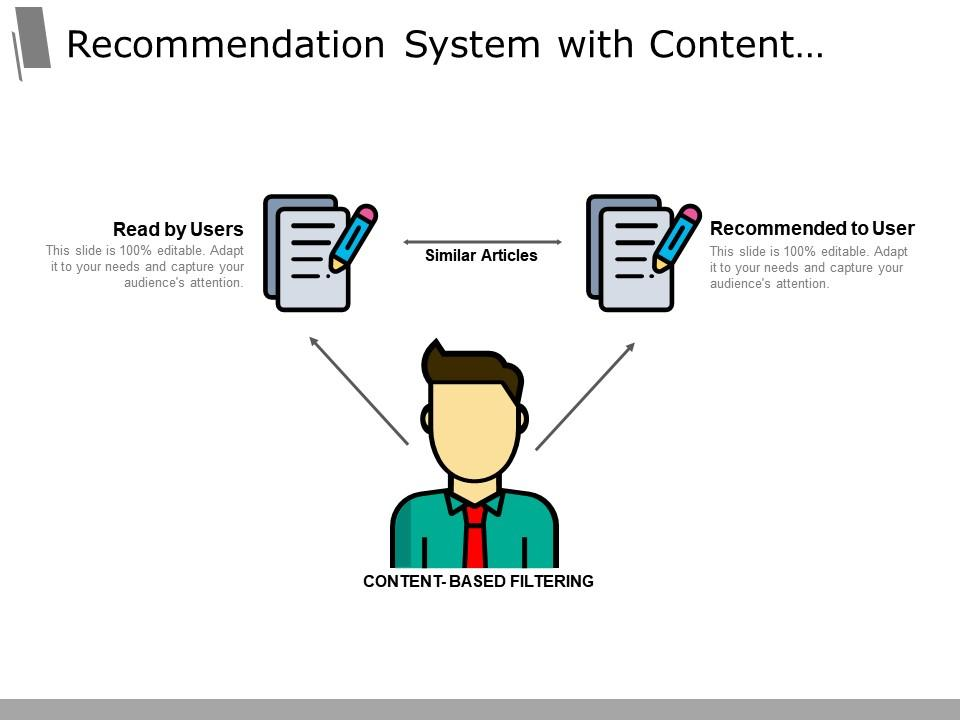
\includegraphics[width=0.8\textwidth]{2}
    \label{fig:img1}
  \end{figure}  
\end{frame}

\begin{frame}{Коллаборативная фильтрация}
  \begin{figure}[H]
    \centering
    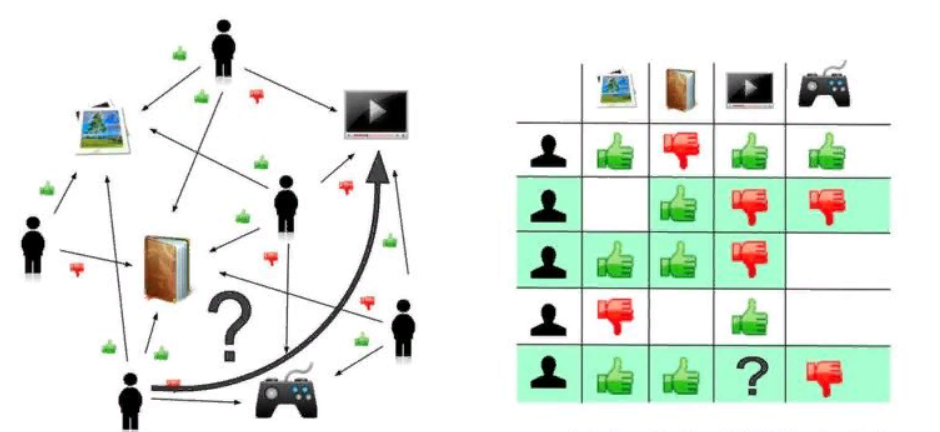
\includegraphics[width=0.8\textwidth]{3}
    \label{fig:img1}
  \end{figure}  
\end{frame}

\begin{frame}{Гибридная фильтрация}
  \begin{figure}[H]
    \centering
    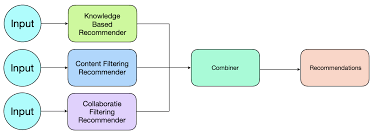
\includegraphics[width=0.7\textwidth]{4}
    \label{fig:img1}
  \end{figure}  
\end{frame}

\begin{frame}{Описание набора данных}
  В качестве основной выборки были использованы данные, предоставленные компанией H\&M для kaggle соревнования по построению рекомендательной системы. Данная выборка
  представляет из себя три таблицы, записанные в формате CSV: таблицу пользователей (customres.csv), содержащую в себе признаки 1371980 пользователей, таблицу объектов (articles.csv),
  содержащую в себе признаки 105542 товаров магазина, и таблицу взаимодействий (transactions.csv), содержащую в себе факты покупки товаров пользователями.  
\end{frame}

\begin{frame}{План работы}
  \begin{enumerate}
    \item Анализ и предобработка данных. Создание новых признаков.
    \item Исследование области рекомендательных систем и выбор алгоритмов машинного обучения.
    \item Обучение моделей и подбор оптимальных гиперпараметов для них.
    \item Оценка качества алгоритмов и анализ результатов.
  \end{enumerate}
\end{frame}

\begin{frame}{Используемые инструменты}
  В качестве языка программирования для данной работы был выбран Python 3.10.10, т.к. он является
  практически безальтернативным решением для работы с машинным обучением.
  
  Для проведения экспериментов с моделями и анализ данных была использована платформа Jupyter Notebook.

  Для визуализации, анализа и предобработки данных были использованы библиотеки matplotlib, seaborn и pandas.

  Для работы с моделями были использованы библиотеки implicit и LightFM, которые содержат модели для построения рекомендательных систем разных типов.
\end{frame}

\begin{frame}{Анализ данных}
  \begin{figure}
    \begin{subfigure}{.5\textwidth}
      \centering
      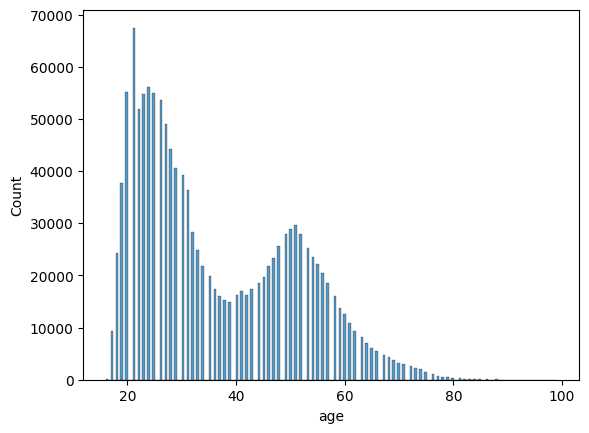
\includegraphics[width=.9\linewidth]{6}
      \label{fig:sfig1}
    \end{subfigure}%
    \begin{subfigure}{.5\textwidth}
      \centering
      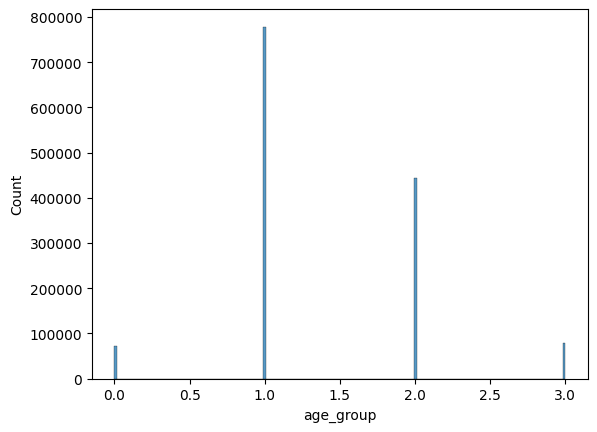
\includegraphics[width=.9\linewidth]{7}
      \label{fig:sfig2}
    \end{subfigure}
    \begin{subfigure}{.5\textwidth}
      \centering
      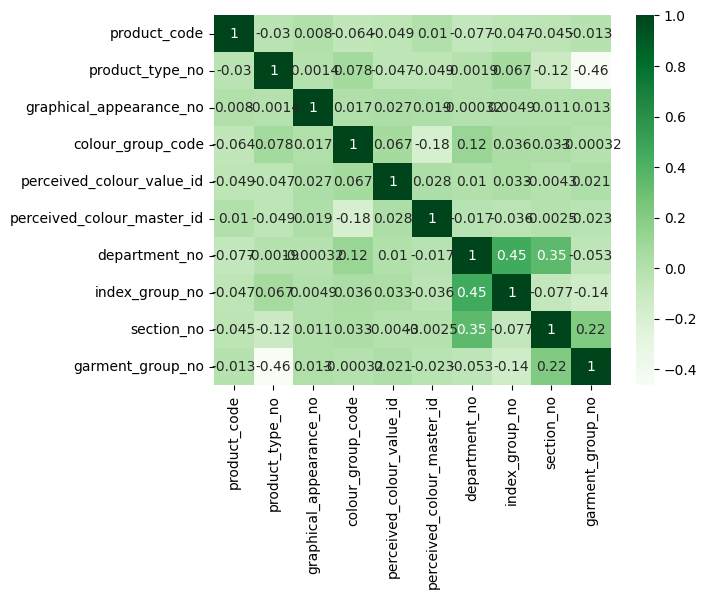
\includegraphics[width=.8\linewidth]{8}
      \label{fig:sfig3}
    \end{subfigure}
    \label{fig:fig}
    \end{figure}
\end{frame}

\begin{frame}{Анализ данных}
  \begin{figure}
    \begin{subfigure}{.4\textwidth}
      \centering
      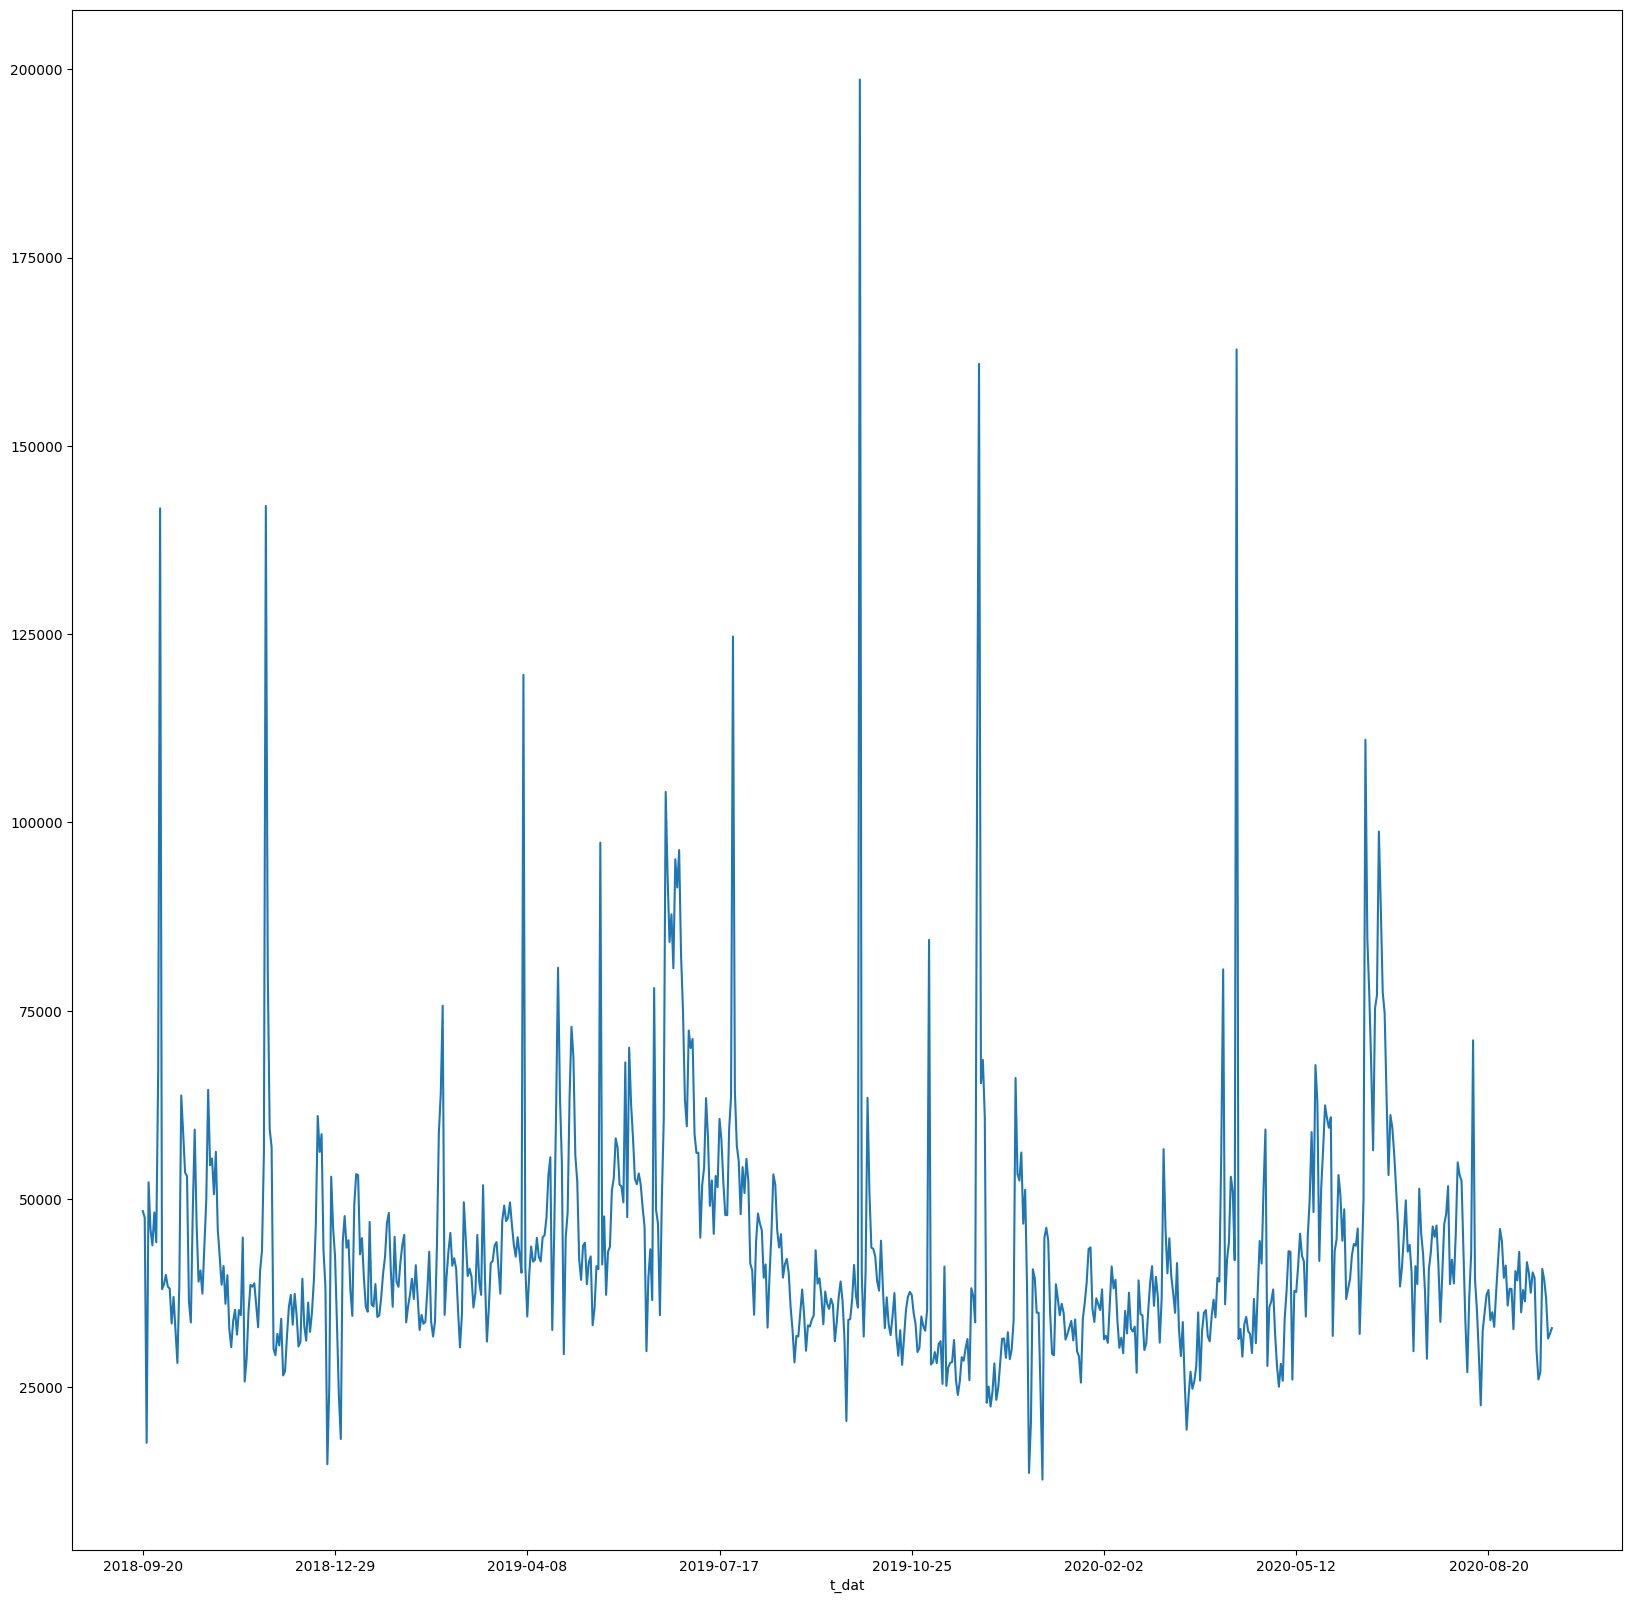
\includegraphics[width=.9\linewidth]{9}
      \label{fig:sfig1}
    \end{subfigure}%
    \begin{subfigure}{.5\textwidth}
      \centering
      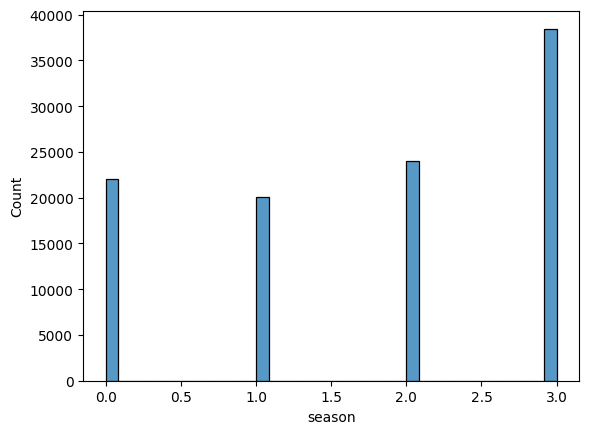
\includegraphics[width=.9\linewidth]{10}
      \label{fig:sfig2}
    \end{subfigure}
    \begin{subfigure}{.5\textwidth}
      \centering
      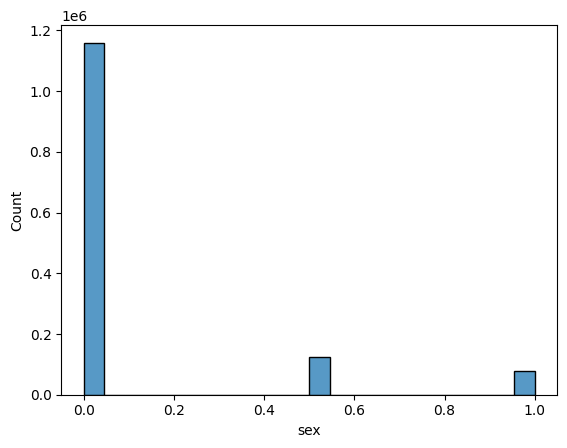
\includegraphics[width=.8\linewidth]{11}
      \label{fig:sfig3}
    \end{subfigure}
    \label{fig:fig}
    \end{figure}
\end{frame}

\begin{frame}{Используемые модели}
  В качестве бейзлайн модели была взята рекомендация популярного, который дальше был модифицирован с помощью нескольких простых правил:
  рекомендации популярного относительно целевой группы пользователя и его пола.

  В качестве модели, основанной на контенте была взята модель tf-idf из библиотеки implicit.

  Для матричного разложения были использованы модели ALS из библиотеки implicit и LightFM из одноименной библиотеки.
  Причем LightFM может также являться гибридной, так как это разложение может учитывать признаки пользователей и объектов. 
\end{frame}

\begin{frame}{Результаты обучения}
  В качестве целевой метрики была выбрана метрика MAP$@12$, так как данная метрика является целевой в данном соревнование.

  \begin{equation}
    \text{p}@k = \frac{\text{количество релевантных элементов}}{k}.
  \end{equation}
  \begin{equation}
    \text{ap}@k = \frac{1}{k}\sum_{i=1}^{k}r_i\text{p}@i,
  \end{equation}
  где $r_i$ принимает значение 1, в случае если $i$ элемент топа является релевантным, и 0 в обратном случае.
  \begin{equation}
    \text{map}@k = \frac{1}{n}\sum_{i=1}^{n}\text{ap}@k_j.
  \end{equation}
\end{frame}

\begin{frame}{Результаты обучения}
  Валидация моделей проводилась на последней неделе тренировочной выборки. А в качестве тестовой использовались закрытые данные,
  на которых тестовая система соревнования оценивает качество прогноза моделей. Которая в свою очередь поделена на две части в
  соотношении 1 к 99. Ее наименьшая часть называется public, а наибольшая "--- private, за счет чего можно сравнить скорость
  деградации моделей.

  Результаты обучения моделей приведены в таблице 1.
\end{frame}

\begin{frame}{Результаты обучения}
  \begin{figure}[H]
    \centering
    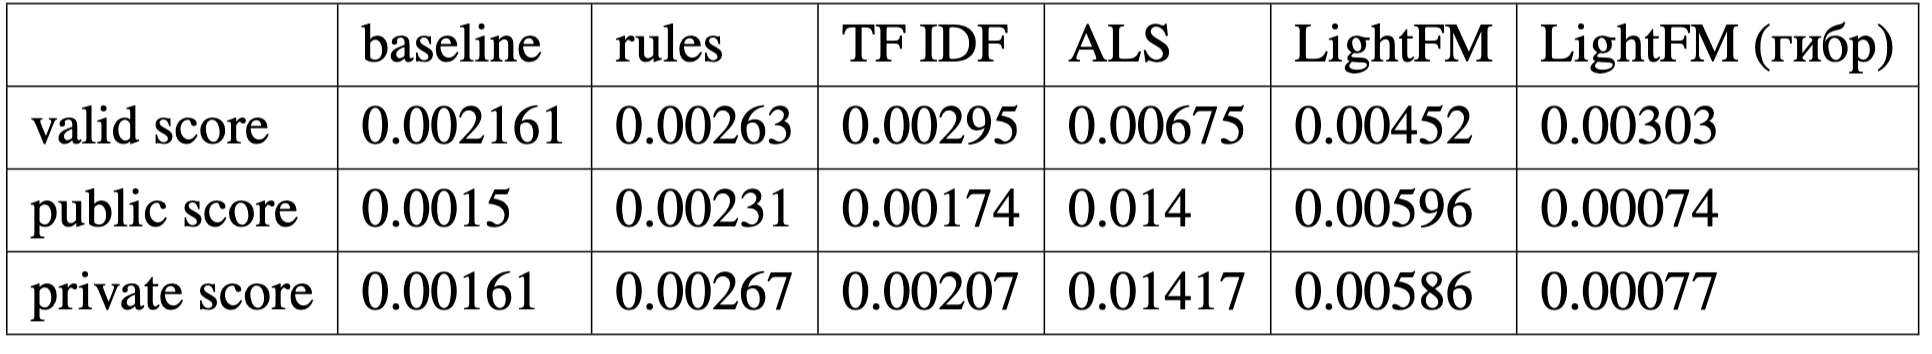
\includegraphics[width=1.\textwidth]{pic/5}
    \label{fig:img1}
  \end{figure}
\end{frame}

\begin{frame}{Выводы}
  По результатам, которые выдали модели можно сделать следующие выводы:
\begin{enumerate}
    \item Модели, основанные на рекомендации популярного очень быстро деградируют, однако этот минус нивелируется
    тем, что их не нужно обучать. Достаточно просто рассчитывать, какие товары находятся в тренде в данный момент времени
    с помощью одного запроса в базу данных.
    \item Усложнив запрос в базу данных несколькими простыми правилами, можно сильно поднять качество бейзлайна.
    \item Модели матричной факторизации дают лучшие метрики относительно любых моделей первого уровня, однако работают плохо
    с холодными пользователями и объектами.
    \item Гибридные модели первого уровня показывают себя намного хуже, чем любые другие модели первого уровня, при этом усложняя
    программную реализацию и расходуют больше времени на обучение.
\end{enumerate}
\end{frame}

\begin{frame}{Список использованных источников}
  \begin{enumerate}
    \item Нейронные сети для начинающих. Часть 1 [Электронный ресурс] – URL: https://habr.com/ru/post/312450/ (дата обращения 13.05.2022) - Загл. с экрана. Яз. рус.
    \item Verma Y. <<A Guide to Building Hybrid Recommendation Systems for Beginners>> [Электронный ресурс] – URL: https://analyticsindiamag.com/a-guide-to-building-hybrid-recommendation-systems-for-beginners/ (дата обращения 01.05.2023) - Загл. с экрана. Яз. англ.
    \item Ермилов Д. <<Рекомендательные системы: продвинутые алгоритмы>> [Электронный ресурс] – URL: https://www.bigdataschool.ru/blog/recommender-systems-advanced-algorithms.html (дата обращения 01.05.2023) - Загл. с экрана. Яз. рус.
  \end{enumerate} 
\end{frame}

\begin{frame}
  \begin{enumerate}
    \setcounter{enumi}{3}
    \item Коллаборативная фильтрация простыми словами [Электронный ресурс] – URL: https://lala.lanbook.com/kollaborativnaya-filtraciya-prostymi-slovami (дата обращения 01.05.2023) - Загл. с экрана. Яз. рус.
    \item Метрики качества ранжирования [Электронный ресурс] – URL: https://habr.com/ru/companies/econtenta/articles/303458/ (дата обращения 01.05.2023) - Загл. с экрана. Яз. рус.
    \item Pykes K. <<Normalized Discounted Cumulative Gain>> [Электронный ресурс] – URL: https://towardsdatascience.com/normalized-discounted-cumulative-gain-37e6f75090e9 (дата обращения 01.05.2023) - Загл. с экрана. Яз. англ.
    \item Park M., Lee K. <<Exploiting Negative Preference in Content-based Music Recommendation with Contrastive Learning>> [Статья] Яз. англ.
    \item Recommendation system with content based filtering [Электронный ресурс] – URL: https://www.slideteam.net/recommendation-system-with-content-based-filtering.html (дата обращения 01.05.2023) - Загл. с экрана. Яз. англ.
  \end{enumerate}
\end{frame}

\begin{frame}
  \begin{enumerate}
    \setcounter{enumi}{8}
    \item Building a hybrid recommendation system for Jokes recommendations [Электронный ресурс] – URL: https://www.oreilly.com/library/view/advanced-machine-learning/9781838641771/0aa25981-d582-4347-9928-2d967133822e.xhtml (дата обращения 01.05.2023) - Загл. с экрана. Яз. англ.
    \item Документация matplotlib [Электронный ресурс] – URL: https://matplotlib.org (дата обращения 12.05.2022) Яз. англ.
    \item Документация seaborn [Электронный ресурс] – URL: https://seaborn.pydata.org (дата обращения 12.05.2022) Яз. англ.
    \item Документация pandas [Электронный ресурс] – URL: https://pandas.pydata.org (дата обращения 12.05.2022) Яз. англ.
    \item Документация implicit [Электронный ресурс] – URL: https://implicit.readthedocs.io/en/latest/quickstart.html (дата обращения 12.05.2022) Яз. англ.
    \item Документация LightFM [Электронный ресурс] – URL: https://making.lyst.com/lightfm/docs/home.html (дата обращения 12.05.2022) Яз. англ.
  \end{enumerate}
\end{frame}

  \begin{frame}
    \begin{beamercolorbox}[ht=7ex, dp=4ex, center, shadow=true, rounded=true]{title in head/foot}
    \centerline{\LARGE{СПАСИБО ЗА ВНИМАНИЕ!}}
    \end{beamercolorbox}
  \end{frame}

\end{document}
